%! Author = maxwe
%! Date = 12.01.23

% Preamble
\documentclass{scrartcl}

% Packages
\usepackage{amsmath}
\usepackage{graphicx}
\usepackage{biblatex}
\usepackage{tabularray}
\UseTblrLibrary{booktabs}

\usepackage{symbols}
\usepackage{hyperref}

% Document
\begin{document}

    \title{Documentation for the pyroll-thermal-2d Plugin}
    \author{Max Weiner}
    \date{\today}

    \maketitle


    \section{Model Description}\label{sec:model-description}

    \begin{figure}
        \centering
        \includegraphics[scale=0.8]{img/heat_flow}
        \caption{Heat Flows on a Disk Element Ring}
        \label{fig:heat_flow}
    \end{figure}

    \subsection{Ring Model}

    The following derivations are based on the ring model approach.
    For details on this approach read also the respective documentation\footnote{https://github.com/pyroll-project/pyroll-ring-model}.

    \subsection{Heat Flow Balance}

    see \autoref{fig:heat_flow}, $\RingIndex$ index of layer in radial direction, $\DiskIndex$ index of disk element in x-direction

    \begin{equation}
        0 = \HeatFlow_1 - \HeatFlow_2 - \HeatFlow_3 + \HeatFlow_4 + \HeatSource
        \label{eq:heat_flow_balance}
    \end{equation}

    heat flow contributions

    \begin{equation}
        \HeatFlow_1 = \Density \ThermalCapacity \VolumeFlow_\RingIndex \Temperature_{\RingIndex}^{\DiskIndex}
        \label{eq:heat_flow_1}
    \end{equation}

    \begin{equation}
        \HeatFlow_2 = \Density \ThermalCapacity \VolumeFlow_\RingIndex \Temperature_{\RingIndex}^{\DiskIndex+1}
        \label{eq:heat_flow_2}
    \end{equation}

    \begin{equation}
        \HeatFlow_3 = -\ThermalConductivity \frac{\Temperature_{\RingIndex+1}^{\DiskIndex}-\Temperature_{\RingIndex}^{\DiskIndex}}{\Radius_{\RingIndex+1} - \Radius_{\RingIndex}} \times 2 \pi \RadiusBoundary_{\RingIndex+1} \XWidth
        \label{eq:heat_flow_3}
    \end{equation}

    \begin{equation}
        \HeatFlow_4 = -\ThermalConductivity \frac{\Temperature_{\RingIndex}^{\DiskIndex}-\Temperature_{\RingIndex-1}^{\DiskIndex}}{\Radius_{\RingIndex} - \Radius_{\RingIndex - 1}} \times 2 \pi \RadiusBoundary_{\RingIndex} \XWidth
        \label{eq:heat_flow_4}
    \end{equation}

    \begin{equation}
        \HeatSource = \HeatSourceEfficiency \frac{\FlowStress}{\FormingEfficiency} \StrainRate \Volume
        \label{eq:heat_source}
    \end{equation}

    where the volume flow $\VolumeFlow$

    \begin{equation}
        \VolumeFlow_\RingIndex = \CrossSection_{\RingIndex} \frac{\XWidth}{\TimeWidth}
        \label{eq:volume_flow}
    \end{equation}

    \begin{equation}
        \CrossSection_{\RingIndex} = \pi \left( \RadiusBoundary_{\RingIndex+1}^2 -  \RadiusBoundary_{\RingIndex}^2 \right)
        \label{eq:cross_section}
    \end{equation}

    at surface different $\HeatFlow_3$, with surface temperature $\SurfaceTemperature$

    \begin{equation}
        \HeatFlow_3 = \left[ -\HeatTransferCoefficient \left( \EnvironmentTemperature - \SurfaceTemperature \right) - \RadiationCoefficient\RelativeRadiationCoefficient\left( \EnvironmentTemperature^4 - \SurfaceTemperature^4 \right) \right]
        \times 2 \pi \RadiusBoundary_{\RingIndexMax+1} \XWidth
        \label{eq:heat_flow_3_surface}
    \end{equation}

    surface temperature estimation as stationary state between environment and outer layer, numerical solution

    \begin{equation}
        \ThermalConductivity \frac{\SurfaceTemperature - \Temperature_\RingIndexMax^\DiskIndex}{\RadiusBoundary_{\RingIndexMax+1} - \Radius_{\RingIndexMax}} = \HeatTransferCoefficient \left( \EnvironmentTemperature - \SurfaceTemperature \right) + \RadiationCoefficient\RelativeRadiationCoefficient\left( \EnvironmentTemperature^4 - \SurfaceTemperature^4 \right)
        \label{eq:surface_temperature}
    \end{equation}

    \subsection{Temperature Increment Functions}

    for core layer $\HeatFlow_4 = 0$

    \begin{equation}
        \TemperatureIncrement_0 = \frac{\TimeWidth}{\Density\ThermalCapacity\CrossSection_0} \left[ \pi \ThermalConductivity \left( \Temperature_1^\DiskIndex - \Temperature_0^\DiskIndex \right) + \HeatSourceEfficiency \frac{\FlowStress}{\FormingEfficiency} \StrainRate \CrossSection_0 \right]
        \label{eq:increment_core}
    \end{equation}

    for intermediate layers with \autoref{eq:heat_flow_3}

    \begin{equation}
        \TemperatureIncrement_\RingIndex = \frac{\TimeWidth}{\Density\ThermalCapacity\CrossSection_\RingIndex}
        \left[
        2 \pi \ThermalConductivity \left[
            \frac{\Temperature_{\RingIndex+1}^\DiskIndex - \Temperature_\RingIndex^\DiskIndex}{\Radius_{\RingIndex+1}-\Radius_{\RingIndex}}
            \RadiusBoundary_{\RingIndex+1}
            -\frac{\Temperature_{\RingIndex}^\DiskIndex - \Temperature_{\RingIndex-1}^\DiskIndex}{\Radius_{\RingIndex}-\Radius_{\RingIndex-1}}
            \RadiusBoundary_{\RingIndex}
            \right]
        + \HeatSourceEfficiency \frac{\FlowStress}{\FormingEfficiency} \StrainRate \CrossSection_{\RingIndex}
        \right]
        \label{eq:increment_layer}
    \end{equation}

    for surface layer with \autoref{eq:heat_flow_3_surface}

    \begin{equation}
        \TemperatureIncrement_\RingIndexMax = \frac{\TimeWidth}{\Density\ThermalCapacity\CrossSection_\RingIndexMax}
        \left[
        2 \pi \left[
            \left[ \HeatTransferCoefficient \left( \EnvironmentTemperature - \SurfaceTemperature \right) + \RadiationCoefficient\RelativeRadiationCoefficient\left( \EnvironmentTemperature^4 - \SurfaceTemperature^4 \right) \right]
           \RadiusBoundary_{\RingIndexMax+1}
            -\ThermalConductivity \frac{\Temperature_{\RingIndexMax}^\DiskIndex - \Temperature_{\RingIndexMax-1}^\DiskIndex}{\Radius_{\RingIndexMax}-\Radius_{\RingIndexMax-1}}
            \RadiusBoundary_{\RingIndexMax}
            \right]
        + \HeatSourceEfficiency \frac{\FlowStress}{\FormingEfficiency} \StrainRate \CrossSection_{\RingIndexMax}
        \right]
        \label{eq:increment_surface}
    \end{equation}


    \section{Plugin Usage}\label{sec:plugin-usage}

    \addsec{Symbols}

\begin{longtblr}[
    label= none,
    entry = none
]{ll}
    \toprule
    Symbol & Description \\
    \midrule
    
    ${{s["code"]}}$ & {{s["descr"]}}\\
    
    \bottomrule
\end{longtblr}

    \printbibliography


\end{document}